\chapter{Outro Cap}
\label{chapter:cap4}

\section{\textbf{Introdução}}
Neste capítulo apresenta-se uma classificação dos métodos de localização bidimensional de MS em redes de telefonia móvel celular. Esta classificação simplificada utiliza apenas três critérios: o método de cálculo, o grau de participação do MS no cálculo de posição e o número mínimo de setores requerido para 

\section{\textbf{Conceitos Básicos}}
\label{sec:Cap1Conceitos}

Alguns conceitos que serão utilizados na descrição dos métodos de localização precisam ser previamente definidos.


\begin{figure}[H]
\begin{center}
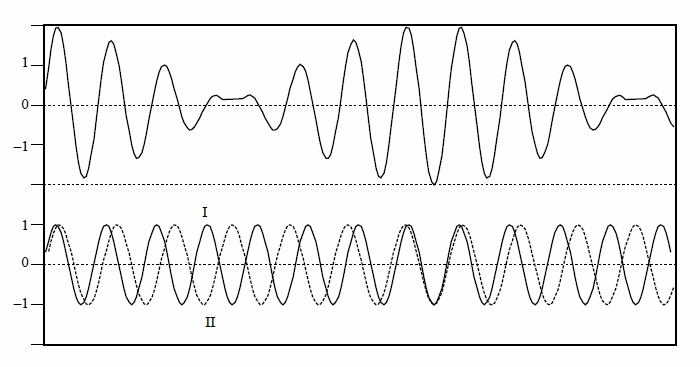
\includegraphics[width=8cm,height=6.4cm]{./01_Cap1/figures/fig_06_br.png}
\caption{\label{fig:bestserverarea}- Áreas Preditas de Melhor Servidor de Três Setores.}
\end{center}
\end{figure}

\section{\textbf{Classificação segundo o Método de Cálculo}}
\label{sec:Cap1Metodo}

O primeiro critério de classificação é a maneira pela qual os métodos de localização calculam a estimativa de posição do MS no plano. Para utilizar a geometria euclidiana, é necessário que as coordenadas geográficas dos setores de referência e do MS sejam representadas através uma projeção cartográfica retangular, ou 

\subsection{Identidade da Célula}
\label{subsec:Cap1Cid}

No método de localização da identidade da célula~(CID - \textit{Cell Identity}), a posição do MS é assumida como sendo igual à da antena transmissora do setor melhor servidor. O método CID, embora seja de baixa complexidade e elevada 

\subsection{Triangulação}
\label{subsec:Cap1Triangulacao}

As técnicas de triangulação utilizam medidas de distâncias~(multi-lateração) ou ângulos~(multi-angulação) entre o MS e os setores de referência para estimar a localização do 

Todos os métodos de triangulação presumem condições de propagação com linha de visada~(LOS - \textit{Line of Sight}) entre o MS e setores de referência. A propagação por múltiplos percursos e a presença de obstáculos entre o MS e os setores de referência podem corromper as medidas angulares, de tempo e de atenuação no percurso. Assim, a propagação sem linha de visada~(NLOS - \textit{Non Line of Sight}) é a principal fonte de erro para esses métodos. Como a propagação NLOS predomina em ambientes urbanos, a precisão dos métodos de triangulação pode ser seriamente comprometida nesses ambientes.

Além da propagação NLOS, outro fator que limita a precisão dos métodos de triangulação é a resolução finita das medidas realizadas na interface aérea e que são utilizadas no cálculo de posição: tempo, RSS e ângulo de chegada. A resolução da medida de RSS depende de especificações da interface rádio. Em redes GSM e WCDMA, por exemplo, os valores de RSS são reportados pelo MS em passos de $1$ dB~\cite{MURRAY}
\begin{equation}
\label{eq:dist}
\hat{d}_{i}= \frac{c \cdot \textrm{T}_{s} \cdot \textrm{RTT}_{i}}{2}
\end{equation}


\begin{table}[ht]
\centering
\caption{\label{tab:quadrosinotico}- Quadro Sinótico dos Métodos de Localização.}
\vspace*{.1cm}
\begin{scriptsize}
\begin{tabular}{|c|c|c|c|c|c|}
\hline
\textbf{Sigla} & \textbf{Método de Cálculo} & \textbf{Participação} & \textbf{Quant. Mín.} & \textbf{Elem. adicionais} & \textbf{Requer}\\
& & \textbf{do MS} & \textbf{de Setores} & \textbf{na RAN} & \textbf{LOS ?}\\
\hline
AOA	& Triang. por multi-angulação & Baseado & 2	& Conj. de antenas & Sim \\
& & na Rede & & diretivas & \\
\hline
CID	& Identidade da célula	& Baseado & 1	& - & Não\\
& & na Rede & & & \\
\hline
EOTD	& Triang. por multi-lateração &	Assistido ou &	3	& LMUs & Sim \\
& hiperbólica & Baseado no MS & & & \\
\hline
AGPS	& Triang. por multi-lateração & Assistido & 3 & - & Sim \\
& circular & pelo MS & & & \\
\hline
CID+RTT	& Triang. por multi-lateração &	Baseado & 3	& - & Sim \\
& circular com RTT & na Rede & & & \\
\hline
CID+RSS	& Triang. por multi-lateração circular  &	Baseado & 3	& - & Sim \\
& com perda de propagação & na Rede & & & \\
\hline
AOA+RTT	& Híbrido	& Baseado & 1	&  Conj. de antenas & Sim \\
& & na Rede & & diretivas & \\
\hline
AOA+RSS	& Híbrido	& Baseado & 1	&  Conj. de antenas & Sim \\
& & na Rede & & diretivas& \\
\hline
AOA+TDOA	& Híbrido	& Assistido & 2	&  Conj. de antenas & Sim \\
& & pelo MS & & diretivas& \\
\hline
\end{tabular}
\end{scriptsize}
\vspace*{-.2cm}
\end{table}


